\section{Silent Failures}
\label{sec:failures}

Several times during development, one of our judges failed without raising an
error, or nearly did. Table~\ref{tab:failures} lists six cases. Two produced a
leaderboard that ranked nothing, which a simple check catches. The others
produced, or would have produced, a leaderboard that still ranked systems, just
less well. We think this is the part of our work that transfers best, because the
score alone gives no hint that anything went wrong.

\begin{table*}
  \caption{Failures that raised no error and what caught each one.}
  \label{tab:failures}
  \small
  \begin{tabular}{@{}p{0.2\textwidth}p{0.33\textwidth}p{0.18\textwidth}p{0.22\textwidth}@{}}
    \toprule
    What failed & What it looked like & What caught it & Fix\\
    \midrule
    The LLM client's default 60\,s timeout and its circuit breaker, which aborts
    the whole batch after 25 failed calls &
    gpt-oss-20b scored 0.000 on rag25-gen. Of 5,302 calls, 26 were slow. That
    threw away all 5,302 judgments, so every measure was constant &
    The 0.000 on TIRA, then a check that found every measure constant. We now run
    that check before every upload &
    A 900\,s timeout, the breaker switched off and our own retries for each call.
    The same run then scored 0.783. A later review found the breaker would
    also have thrown away cached replies during TIRA's replay. So it is off there
    too\\
    \addlinespace
    Client settings that carry over between phases &
    Caught before it touched any run we report. If one connection failed while the
    model server was still loading, a 5\,s timeout could stick for the whole
    judging phase. Long responses would then time out and score zero, yet the
    measures would still vary &
    A code audit hunting for failures that still give a plausible leaderboard &
    Every phase re-applies the settings from a snapshot of the operator's own
    values\\
    \addlinespace
    A reasoning model using up its reply budget mid-thought &
    After the first pass, 27\% of the rag26 judgments by gpt-oss-20b could not be
    read &
    vLLM's own counters, which showed 5,020 of 13,275 requests ending at the
    length limit &
    A larger budget on each retry (Figure~\ref{fig:budget})\\
    \addlinespace
    A single exception that fails the whole batch &
    On the gpt-oss-20b run, one thrown exception took down all 5,302 judgments in
    the batch. The retry changed the prompt, so the cache could not help. On the
    last attempt it would have scored every response zero and logged just one
    warning line &
    The run's log &
    Resend the exact same batch so the cached replies replay\\
    \addlinespace
    A reproducibility check with nothing to reproduce &
    The container rehearsal passed the cache-replay check without making
    any LLM call. The endpoint was a closed port.
    The judge fell back to all-zero scores and the replay reproduced them exactly &
    Reading the rehearsal's output &
    Rehearse against a stub endpoint that actually replies. Then require the
    replayed leaderboard to separate systems\\
    \addlinespace
    A threshold below every observed value &
    \judge{Corroborate}'s specificity floor kept 100\% of clusters. A parameter
    sweep showed no effect (Section~\ref{sec:floor}) &
    Measuring the range of scores the encoder actually gives &
    A floor inside that range. A warning now fires when a filter keeps everything
    or nothing\\
    \bottomrule
  \end{tabular}
\end{table*}

Two patterns run through the table. First, a failure that zeroes everything is easy
to catch. A check that the measures vary across systems will flag it. A failure
that zeroes only some responses slips past, because the leaderboard still ranks
systems. The sticky timeout is the dangerous case. Left in place, it would have
zeroed long responses first. Systems would then rank partly by how short their
responses were. Under the earlier ragtime25 scoring, length alone correlated with
the human ranking at 0.558. That hidden bias could have pulled the score down a
long way with no warning. Second, a reproducibility check compares two runs, so
two runs that both do nothing will pass it. Every sameness check needs a liveness
check beside it, one that confirms the judge did real work.

\begin{figure}
  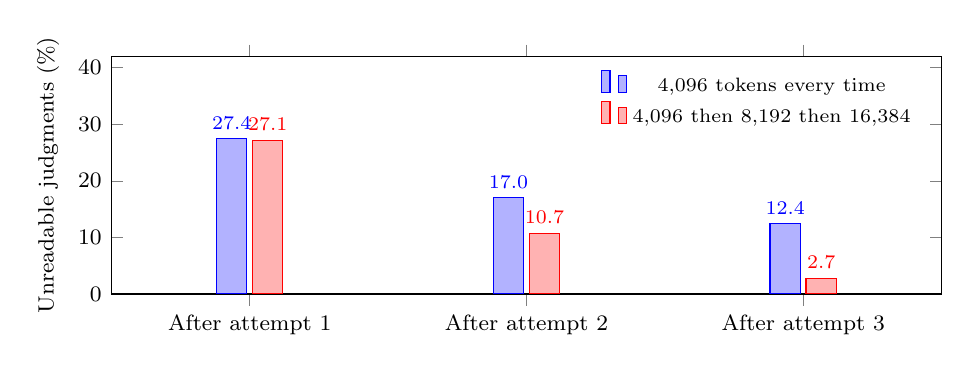
\begin{tikzpicture}
    \begin{axis}[
        ybar,
        width=\columnwidth,
        height=4.6cm,
        bar width=11pt,
        ymin=0, ymax=42,
        ylabel={Unreadable judgments (\%)},
        symbolic x coords={1,2,3},
        xtick=data,
        xticklabels={After attempt 1, After attempt 2, After attempt 3},
        x tick label style={font=\footnotesize},
        y tick label style={font=\footnotesize},
        ylabel style={font=\footnotesize},
        nodes near coords,
        nodes near coords style={font=\scriptsize},
        point meta=explicit symbolic,
        legend style={font=\scriptsize, at={(0.98,0.97)}, anchor=north east, draw=none},
        enlarge x limits=0.25,
      ]
      \addplot coordinates {(1,27.4) [27.4] (2,17.0) [17.0] (3,12.4) [12.4]};
      \addplot coordinates {(1,27.1) [27.1] (2,10.7) [10.7] (3,2.7) [2.7]};
      \legend{{4,096 tokens every time},{4,096 then 8,192 then 16,384}}
    \end{axis}
  \end{tikzpicture}
  \caption{Share of the 9,838 rag26 judgments by gpt-oss-20b that were still
  unreadable after each attempt. One run keeps the reply budget fixed, while the
  other doubles it on each retry. The first attempt gets the same budget in both
  runs. Its result still differs slightly because some answer keys were rebuilt.}
  \label{fig:budget}
\end{figure}

Figure~\ref{fig:budget} shows what the reply budget does. With 4,096 tokens on
every attempt, 12.4\% of the rag26 judgments by gpt-oss-20b were still unreadable
after three attempts. Giving the retries 8,192 and then 16,384 tokens cut this to
2.7\%, or 264 judgments in all. For the second run we also rebuilt the answer keys.
Retries while building a key got the larger budget too. That is why the first
attempt differs slightly between the two runs. The same model had left only
0.75\% of its judgments unreadable on the rag25-gen pilot and 2.9\% on ragtime25.
The problem grew large only on the test data. So retry counts are worth watching
on the test run itself, not just on a pilot. Our second \judge{NuggetRecall} code
submission, \run{grave-node}, carries this fix.

One more trap is not silent, but it is easy to walk into. A TREC qrels file, the
standard file of relevance labels, has four columns separated by whitespace. So does
a leaderboard. TIRA finds the leaderboard by that shape, so a qrels file written
next to it makes the upload fail. For this reason neither of our judges writes a
qrels file. A script also checks every output folder before upload.
